\section{Introduction}
While diffusion models \citep{ho2020denoising,song2020score,sohl2015deep} are now the leading paradigm for generative modeling in continuous domains, recent work has begun to expand their scope to discrete spaces. The prevailing approach, Masked Diffusion Models (MDMs) \citep{shi2024simplified,sahoo2024simple,gat2024discrete}, generates sentences in a non-left-to-right, any-order fashion. Compared to autoregressive models, this any-order generation ability yields substantially faster inference and strong downstream performance on non-casual tasks such as planning \citep{ye2024beyond}, code \cite{nie2025large,dream2025}, and reasoning \citep{nie2024scaling}.

Despite these successes, current MDMs cannot (1) model distributions supported on sequences of \emph{variable length} and (2) insert new tokens during generation (Figure~\ref{fig:main}, left). Both capabilities are natural desiderata for generative models over discrete domains. We therefore ask: \emph{Can we model variable-length data while preserving MDMs' any-order generation power?}

We answer in the affirmative by proposing the \textbf{Flexible  Masked Diffusion Model} (FlexMDM). FlexMDMs start from an empty string and gradually \coloredul{xblue}{insert mask tokens} and then \coloredul{xblue}{unmask} them (Figure~\ref{fig:main}, right). Beyond learning the usual \emph{unmasking} posterior--the distribution of a clean token at masked positions--we introduce an \emph{insertion} expectation: the expected number of tokens to insert conditioned on the current sequence. Crucially, we show that FlexMDM is \xblue{theoretically grounded} (i.e., under perfect training, it samples from the true data distribution) and \xblue{retains the any-order sampling property} of MDMs, thereby directly addressing the question above.
\begin{figure}[t]
\centering
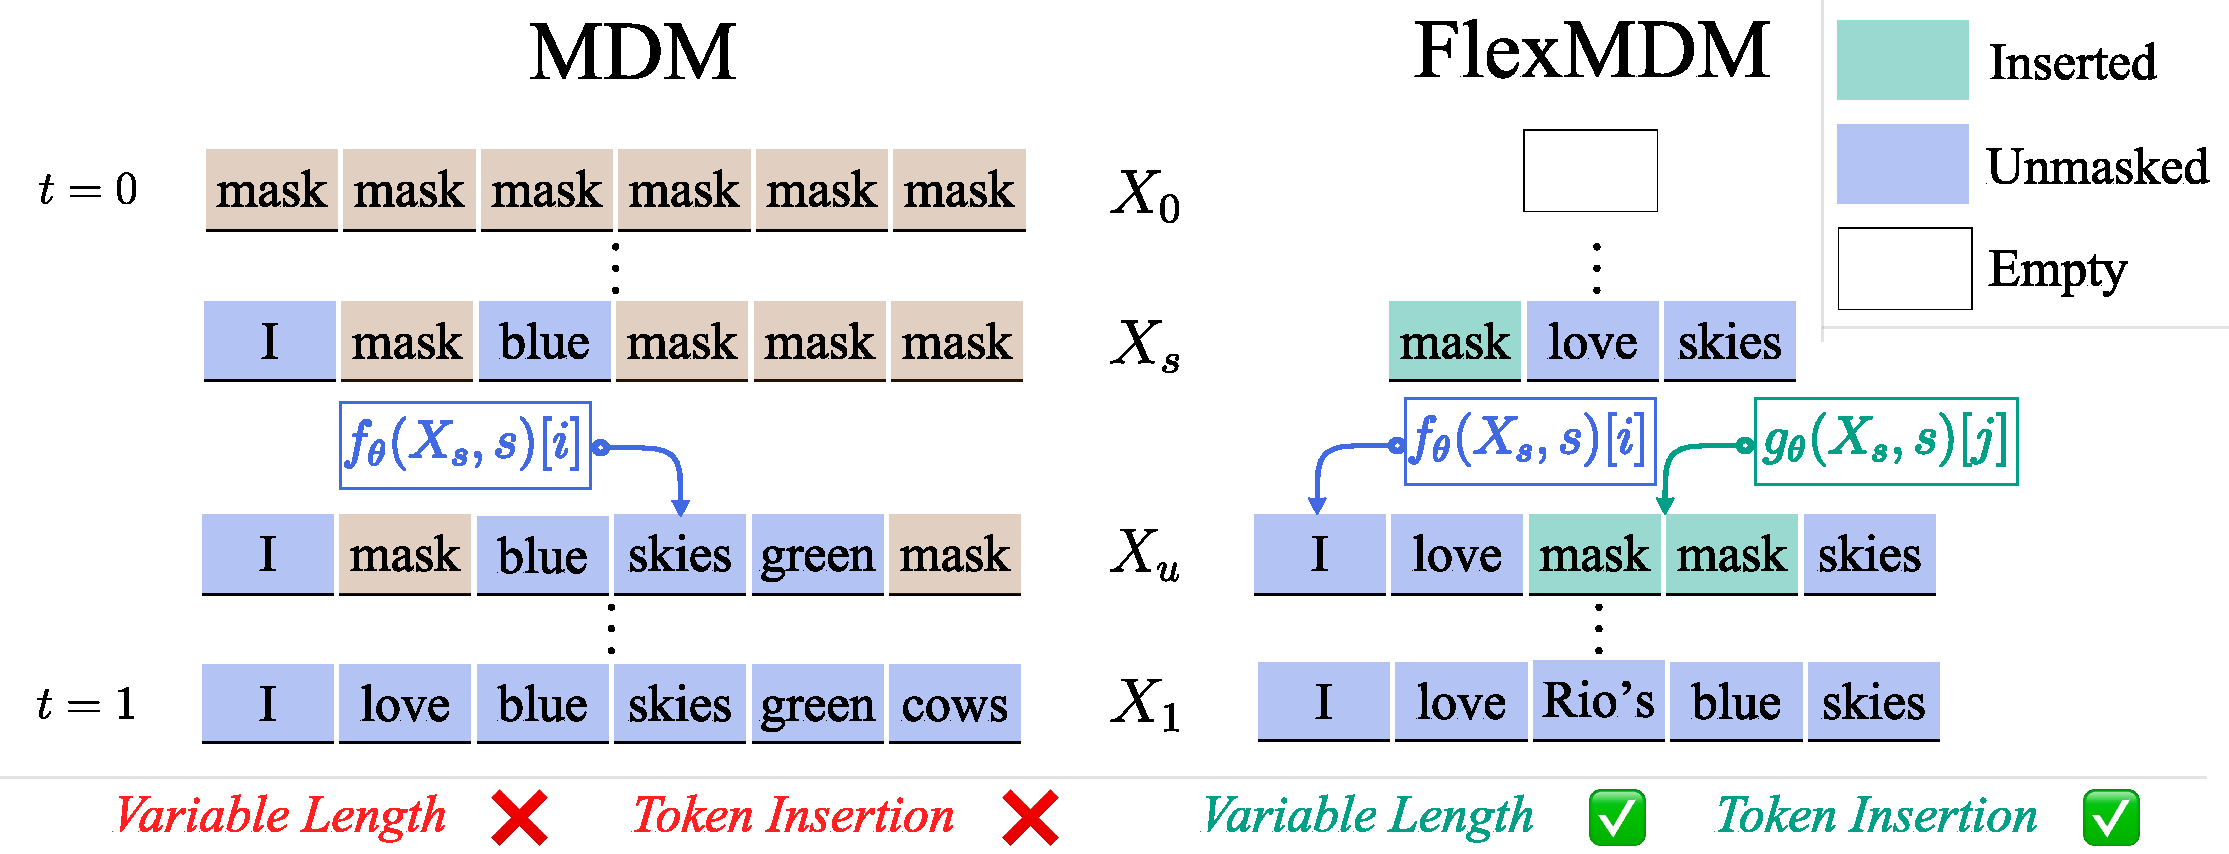
\includegraphics[width=\textwidth,trim={0 0 0 3.0cm}]{Figures/main_fig.pdf}
\caption[Flexible Masked Diffusion Model (FlexMDM)]{%
\textbf{Flexible Masked Diffusion Model} (FlexMDM) \underline{addresses} MDMs’ inability to handle variable-length sequences and token insertion while \underline{preserving} any-order generation power. 
At each step, FlexMDM performs \textbf{\xxgreen{insertion}} and \textbf{\xblue{unmasking}} by predicting \xxgreen{\textbf{the expected number of mask tokens to insert} ($g_\theta$)} and the \xblue{\textbf{posterior over clean tokens} ($f_\theta$)}, respectively.}
\label{fig:main}
\vskip -1.0\baselineskip
\end{figure}
Empirically, we demonstrate that FlexMDM offers significant new upgrades to the MDM paradigm,
\begin{itemize}[leftmargin=*,itemsep=0pt,topsep=-0.25em]
    \item A FlexMDM pretrained on OpenWebText is able to \xxgreen{model the length distribution with substantially higher fidelity} while matching the perplexity of an MDM counterpart. 
    \item On \xxgreen{planning tasks}, FlexMDM achieves markedly better results, beating the success rate of MDMs by nearly 60\% on a natural synthetic baseline. 
    \item \xxgreen{MDMs can be retrofitted into FlexMDMs at 8B+ scale}:  We fine-tune LLaDA-8B \citep{nie2025large}, an open-source MDM, into a FlexMDM using only 16 H100s for three days. The model transfers cleanly from its MDM initialization and, with its newly acquired variable-length capability, attains notably better performance on GSM8K (58\%$\to$67\%) and Code infilling (52\%$\to$65-\%).
\end{itemize}

Theoretically, our construction relies on the machinery of continuous-time Markov chains (CTMCs) and in particular introduces the new notion of a \emph{joint interpolant}, a novel extension of \emph{stochastic interpolants} \citep{albergo2022building, albergo2023stochastic, lipman2022flow}. Recent work~\citep{zheng2024masked,ou2024your} established an equivalence between MDMs and any-order language models--obviating the need for CTMCs. In contrast, we prove that FlexMDMs also possess the flexibility of any-order generation, yet the continuous-time perspective is absolutely essential for them to accurately model the length distribution. Accordingly, we re-derive the connections between MDMs and stochastic interpolants and use them to ground the design of FlexMDMs.




\textbf{Roadmap.} We begin in Section~\ref{sec:pre} with a broadly accessible review of CTMCs and the connection between MDMs and discrete flow matching. Building on this, Section~\ref{sec:FlexMDM_informal} derives the FlexMDM training objective, and Section~\ref{sec:FlexMDM_inference} introduces our inference procedures. Section~\ref{sec:experiment} presents our experimental results.

\textbf{Concurrent work.} Concurrent works \citep{Dreamon2025,havasi2025edit} attempt to tackle the same problem. \cite{Dreamon2025} introduces an auxiliary expand token in training and heuristically replaces each expand token with two mask tokens at inference. \cite{havasi2025edit}, also based on the discrete flow matching framework, shares a similar theoretical grounding as our result. The main differences lie in our particular choice of interpolant that leads to the development of an any-order sampling algorithm. For clarity, we provide a detailed comparison in Appendix~\ref{appendix:related_work}.
